%%%%%%%%%%%%%%%%%%%%%%%%%%%%%%%%%%%%%%%%%%%%%%%%%%%%%%%%%%%%%%%%%%%%%%
% Overleaf (WriteLaTeX) Example: Molecular Chemistry Presentation
%
% Source: http://www.overleaf.com
%
% In these slides we show how Overleaf can be used with standard 
% chemistry packages to easily create professional presentations.
% 
% Feel free to distribute this example, but please keep the referral
% to overleaf.com
% 
%%%%%%%%%%%%%%%%%%%%%%%%%%%%%%%%%%%%%%%%%%%%%%%%%%%%%%%%%%%%%%%%%%%%%%
% How to use Overleaf: 
%
% You edit the source code here on the left, and the preview on the
% right shows you the result within a few seconds.
%
% Bookmark this page and share the URL with your co-authors. They can
% edit at the same time!
%
% You can upload figures, bibliographies, custom classes and
% styles using the files menu.
%
% If you're new to LaTeX, the wikibook is a great place to start:
% http://en.wikibooks.org/wiki/LaTeX
%
%%%%%%%%%%%%%%%%%%%%%%%%%%%%%%%%%%%%%%%%%%%%%%%%%%%%%%%%%%%%%%%%%%%%%%

\documentclass{beamer}

% For more themes, color themes and font themes, see:
% http://deic.uab.es/~iblanes/beamer_gallery/index_by_theme.html
%
\mode<presentation>
{
  \usetheme{Madrid}       % or try default, Darmstadt, Warsaw, ...
  \usecolortheme{default} % or try albatross, beaver, crane, ...
  \usefonttheme{serif}    % or try default, structurebold, ...
  \setbeamertemplate{navigation symbols}{}
  \setbeamertemplate{caption}[numbered]
} 

\usepackage[portuguese]{babel}
\usepackage[utf8x]{inputenc}
\usepackage{chemfig}
\usepackage[version=3]{mhchem}


% On Overleaf, these lines give you sharper preview images.
% You might want to `comment them out before you export, though.
\usepackage{pgfpages}
\pgfpagesuselayout{resize to}[%
  physical paper width=8in, physical paper height=6in]

% Here's where the presentation starts, with the info for the title slide
\title[]{Cidades Inteligentes \& IoT}
\author{Reynaldo Caceres Villena}
\institute{IME-USP}
\date{Junho - 2018}

\begin{document}

\begin{frame}
  \titlepage
\end{frame}

% These three lines create an automatically generated table of contents.
\begin{frame}{Outline}
  \tableofcontents
\end{frame}

































\section{Introdução}
\begin{frame}{Introdução}

\begin{columns}
\begin{column}{0.6\textwidth}
\begin{itemize}
\item No século XIX, 2\% da população mundial morava em cidades. 

\item Com a Revolução Industrial, teve início o processo de
urbanização.
\end{itemize}
\end{column}
\begin{column}{0.4\textwidth}  %%<--- here
    \includegraphics[width=.8\textwidth]{img/campo-city.jpeg}    
\end{column}
\end{columns}





%\begin{alertblock}{}
%Simmons Hall $\not=$ Simmons Dormitory.
%\end{alertblock}
\begin{itemize}

\item Em 2008, 54.6\% ou 3 600 milhões de pessoas, moravam em cidades.
\end{itemize}

\begin{exampleblock}{Dados da ONU - 2015 [R1]}
Em 2050, o 70\% da população mundial (mais de 6 000 milhões) morará
em cidades. 
 
\end{exampleblock}


\end{frame}































































\begin{frame}{Os Grandes Desafios Urbanos}
A nível mundial, as cidades: 
\begin{columns}
\begin{column}{0.7\textwidth}
\begin{itemize}
\item Ocupam somente el 2\% do espaço.
\item Consomem de 60\% a 80\% da energia.
\item Geram o 75\% das emissões de carbono.

\end{itemize}
\end{column}
\begin{column}{0.3\textwidth}  %%<--- here
    \includegraphics[width=.9\textwidth]{img/mundo_ciudad.jpg}    
\end{column}
\end{columns}

\begin{alertblock}{A Elevada Concentração Populacional faz aumentar:}
\begin{itemize}
 \item A poluição do ar e da água.
 \item A geração e disposição dos resíduos sólidos 
 \item O consumo de energia. 
\end{itemize}
E isso afeta de forma considerável ao meio ambiente e ao clima. 



\end{alertblock}


\end{frame}


















































\begin{frame}{Os Grandes Desafios Urbanos }
Uma cidade deve possuir:
\begin{block}{{\bf{Sustentabilidade Meio-Ambiental e Mudança Climática:}}}
\begin{itemize}
 \item  Vinculados ao uso de espaço físico e seus impactos no meio ambiente, assim 
com a capacidade das cidades para antecipar e tomar atitude rapidamente diante de desastres naturais.
\end{itemize}
\end{block}
\begin{center}
    \includegraphics[width=.36\textwidth]{img/mundo_ciudad_contaminacion.jpg}    
\end{center}

 



\end{frame}



















































\begin{frame}{Os Grandes Desafios Urbanos }
Uma cidade deve possuir:
\begin{block}{{\bf{Sustentabilidade Urbana:}}}
\begin{itemize}
 \item  Está associada diretamente com a ocupação das cidades e a habilidade do governo municipal de otimizar os espaços públicos
 e distribuir equitativamente os serviços urbanos. 
 \begin{center}
  \includegraphics[width=.8\textwidth]{img/sustentavel.jpg}
  
 \end{center}

\end{itemize}
\end{block}
        

\end{frame}



















\begin{frame}{Os Grandes Desafios Urbanos }
Uma cidade deve possuir:
\begin{block}{{\bf{Sustentabilidade Fiscal e Governança:}} :}
\begin{itemize}
 \item Deve existir uma gestão pública (habilidade para se comunicar com a população).
 \item Deve existir mecanismos de informação transparente em relação com a administração e as finanças.
 \item Deve existir uma gestão participativa (dados para atuar de acordo com as necessidades) para ter uma eficiência da gestão urbana.
 \begin{center}
  \includegraphics[width=.156\textwidth]{img/guverno1.jpeg}\ \ \ \ \ \ \ \ \ \ \ \ \ \ \ \ \ \ \ \ \ \ \ \ \ \ \ \ 
  \includegraphics[width=.2\textwidth]{img/guverno2.jpeg}
  
 \end{center}

\end{itemize}\end{block}
\end{frame}























\subsection{Cidades Inteligentes}
\begin{frame}{Cidades Inteligentes}

São aquelas cidades que utilizam a tecnologia para ter :
\begin{itemize}
 \item Sustentabilidade de Meio-ambiental e Mudança climática.
 \item Sustentabilidade Urbana.
 \item Sustentabilidade Fiscal e de Governança.
\end{itemize}

 
\begin{center} 
  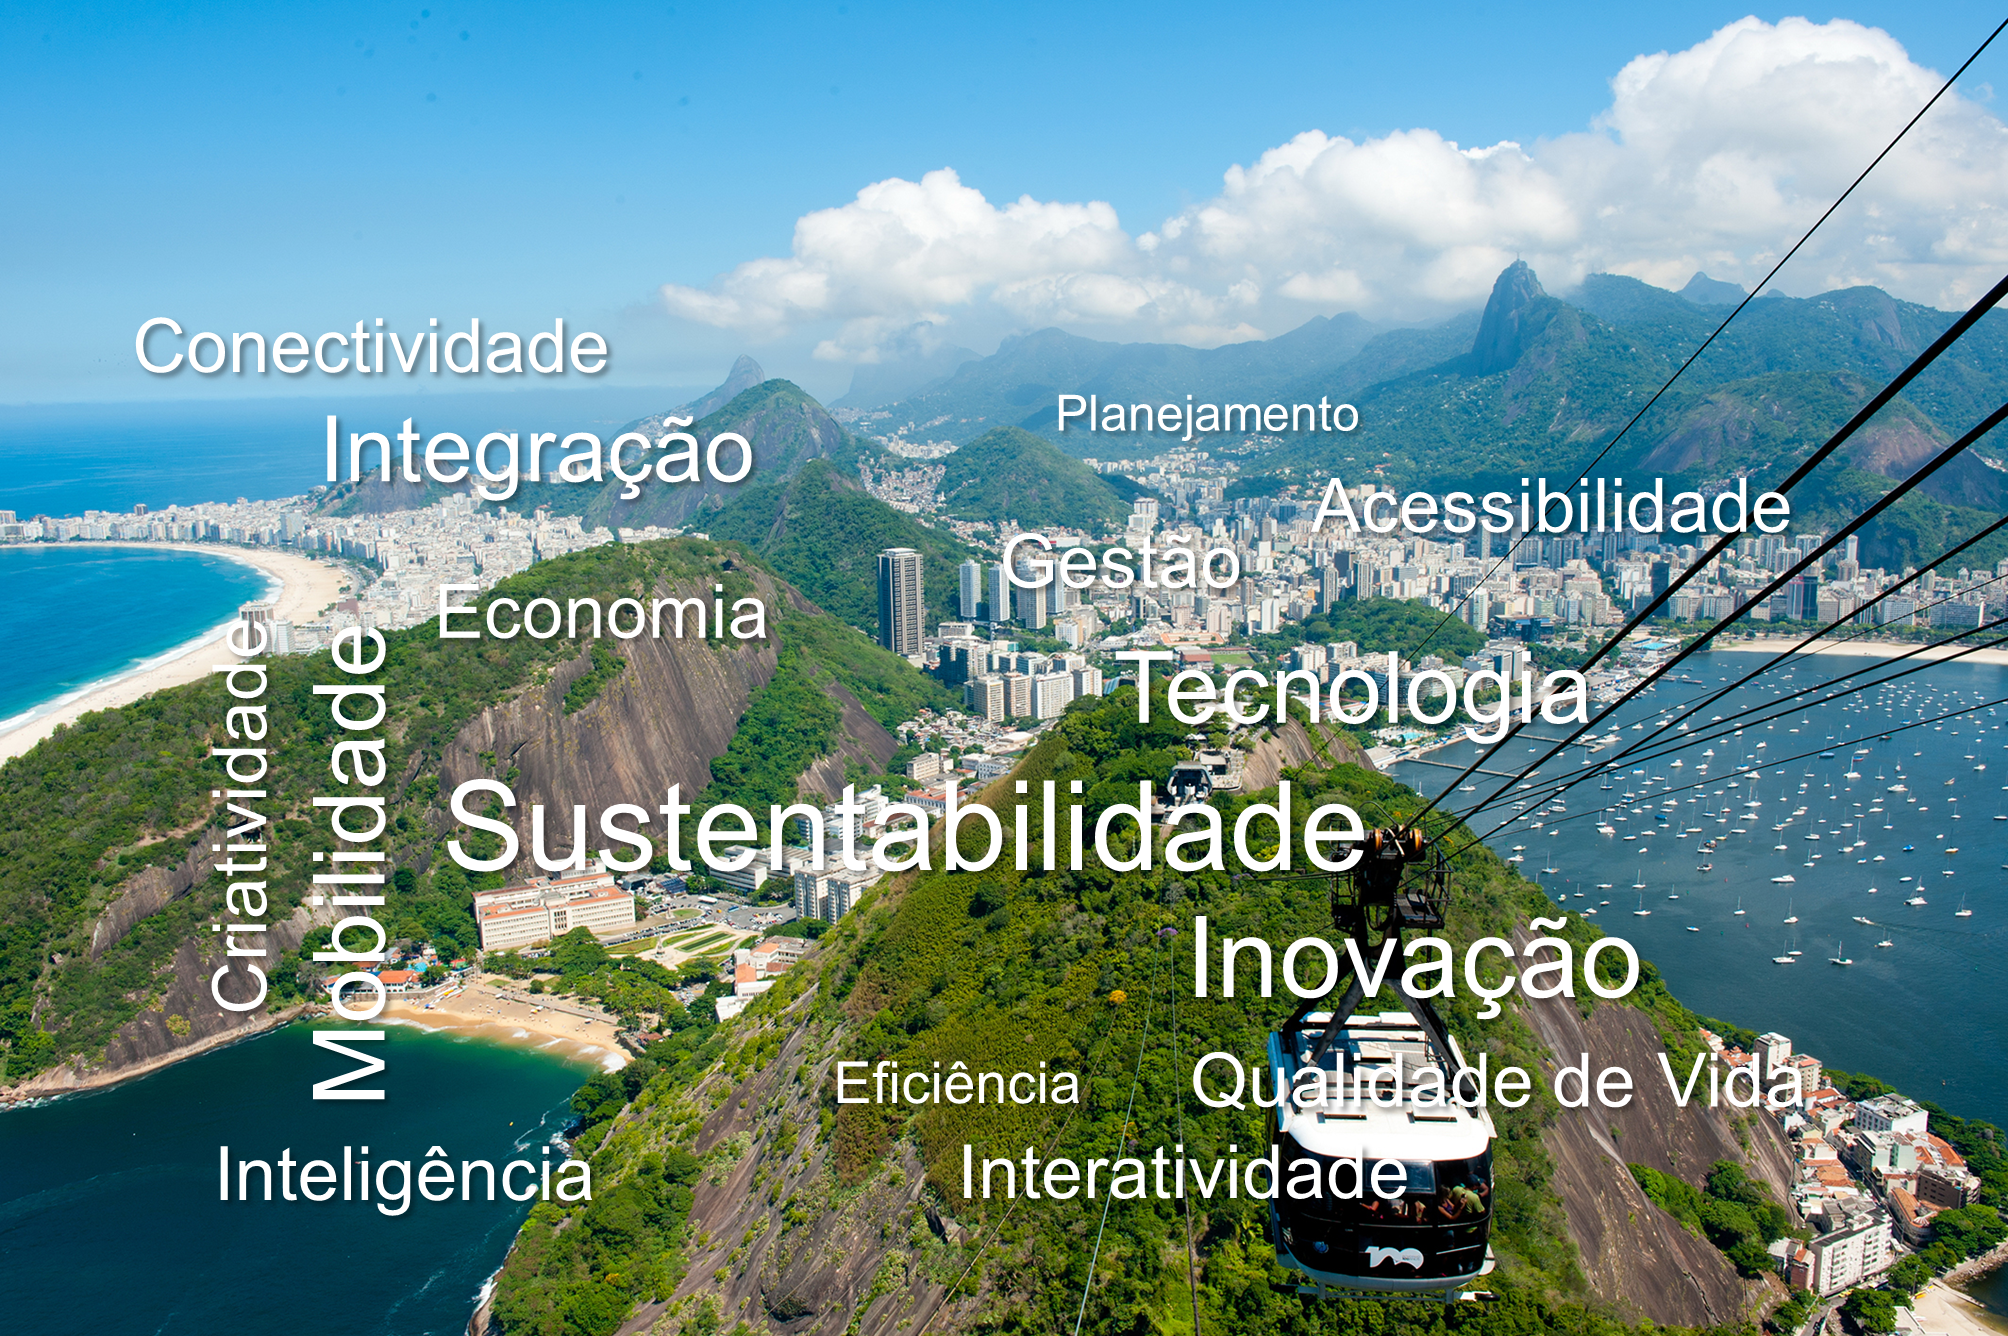
\includegraphics[width=0.6\textwidth]{img/img_cidades_inteligentes.png}
\end{center}

   

\end{frame}































\begin{frame}{Cidades Inteligentes}
Outras Definições:




\begin{columns}
\begin{column}{0.7\textwidth}
\begin{itemize}
 \item São cidades que utilizam avanços tecnológicos para melhorar a qualidade de vida de seus habitantes.
 \item São cidades automatizadas e mais sustentáveis.
\end{itemize}
\end{column}
\begin{column}{0.3\textwidth}  %%<--- here
    \begin{center}
     \includegraphics[width=0.65\textwidth]{img/smart-city.jpg}
     \end{center}
\end{column}
\end{columns}



\begin{columns}
\begin{column}{1\textwidth}
   \begin{itemize}
 \item São aquelas cidades que utilizam tecnologia para gerar eficiência nas operações urbanas, de tal forma que mantém seu desenvolvimento 
  econômico ao mesmo tempo que melhora a qualidade de vida da população.

\end{itemize}
\end{column}
\end{columns}
%\begin{alertblock}{}
%Simmons Hall $\not=$ Simmons Dormitory.
%\end{alertblock}

\end{frame}
















\subsection{IoT- Internet das Coisas}
\begin{frame}{}
\begin{center}
  IoT- Internet das  Coisas

\end{center}

 \end{frame}














\begin{frame}{IoT- Internet das  Coisas }

Internet das Coisas:
\begin{itemize}
 \item Um conceito tecnológico em que todos os objetos da vida cotidiana estariam conectados à internet, agindo de modo inteligente e sensorial (captando estímulos e informações).
\item Tipo de Dispositivos conectados a Internet das Coisas:
\begin{itemize}
 \item Objetos que funcionam como sensores.
 \item Objetos que são controladores ou atuadores.
 
\end{itemize}
\item Cada objeto está conectado à Internet (IP específico), onde pode: 
\begin{itemize}
 \item ser acessado para receber instruções.
 \item enviar os dados coletados para um servidor externo. 
\end{itemize}
\end{itemize} 
\begin{center} 
  \includegraphics[width=0.4\textwidth]{img/IoT.jpg}\ \ \ \ \ \ \ \ \ \ \ 
  \includegraphics[width=0.3\textwidth]{img/IOT3.png}
\end{center}


   

\end{frame}















\begin{frame}{IoT- Internet das Coisas }

\begin{alertblock}{}
 Não é simplesmente colocar uma antena em cada dispositivo e enviar milhões de dados. Os dados devem ser processados e devem ser úteis ao público com aplicações concretas, tangíveis e econômicas.
 \end{alertblock} 
 Exemplos:
 \begin{columns}
\begin{column}{0.55\textwidth}
\begin{itemize}
 \item Relógio inteligente (Apple - 2015): 
 
 \includegraphics[width=.81\textwidth]{img/applewatch.jpg}
\end{itemize}
\end{column}
\begin{column}{0.45\textwidth}
\begin{itemize}
 \item Smart TV
 \item Aplicativos de Segurança
 \item Luzes Inteligentes
 \item Aplicativos de trânsito
 \item Aplicativos de saúde
 \item Wearables fitness
 \item outros
\end{itemize}
\end{column}
\end{columns}


\end{frame}


\section{Cidades Inteligentes \& IoT}
\begin{frame}{Cidades Inteligentes \& IoT}
\begin{block}
 
\begin{itemize}
\item As cidades inteligentes tornam-se possíveis também por meio da
concretização da internet das coisas (IoT). 
\item A IoT aplicado ao ambiente urbano, leva
inteligência a processos já existentes e/ou criam novas
maneiras de se realizar antigas tarefas - e assim surgem
as Cidades Inteligentes.
 
\end{itemize}
\end{block}
\begin{center}
\includegraphics[width=.3\textwidth]{img/IOT4.jpg}\ \ \ \ \ \ \ \ \ \ \ \ \ \ \ \ \  
\includegraphics[width=.3\textwidth]{img/smartcity.png}
 
 
\end{center}


\begin{exampleblock}{} 
``Uma cidade Inteligente é um lugar onde a tecnologia ganha vida''
\end{exampleblock}

\end{frame}




















































\begin{frame}{Uma Cidade Inteligente debe ser:}
\begin{block}
 
\begin{itemize}
\item {\bf{É sustentável:}} Reduze custos e otimizar o consumo de recurso.. 
\item {\bf{É inclusiva e transparente:}} Tem comunicação direta com os cidadãos.
\item {\bf{Gera riqueza:}} Oferece infraestrutura adequada.
\item {\bf{É feito para os cidadãos:}} Melhorar a qualidade de vida das pessoas e da acesso rápido a serviços públicos mais eficientes.

\end{itemize}
\end{block} 

\begin{center}
\includegraphics[width=1\textwidth]{img/focos.png}  
\end{center}



\end{frame}



















































\subsection{Arquitetura de uma Cidade Inteligente}

\begin{frame}{Arquitetura de uma Cidade Inteligente}
\begin{center}
\includegraphics[width=.8\textwidth]{img/arquitetura.png}  
\end{center}
{\tiny{Imagem do texto: [R3]}}


\end{frame}











\begin{frame}{Arquitetura de uma Cidade Inteligente}
\begin{center}
\includegraphics[width=1\textwidth]{img/arquitetura-menu-1.png}  
\end{center}
\begin{exampleblock}{}
Redes de Internet de banda larga (fixas e/ou móveis), para receber e enviar dados.

\begin{itemize}
\item A infraestrutura de comunicação é uma combinação de diferentes tecnologias de rede de dados que usam transmissão via cabos, fibra ótica e redes
sem fio (Wi-Fi, 3G, 4G ou rádio)
\end{itemize}
\end{exampleblock}
\begin{center}
\includegraphics[width=.4\textwidth]{img/internet.jpg}\ \ \ \ \ \ \ \ \ \ \ \ 
\includegraphics[width=.4\textwidth]{img/Internet3.jpg}  
\end{center}



\end{frame}


\begin{frame}{Arquitetura de uma Cidade Inteligente}
\begin{center}
\includegraphics[width=1\textwidth]{img/arquitetura-menu-2.png}  
\end{center}
\begin{exampleblock}{}

 Que captam diferentes sinais do ambiente e os transmitem pelas redes para os computadores nos centros de controle e gerenciamento das cidades, que integram diferentes áreas temáticas, como
trânsito, segurança, atenção ao público, situações de emergência e alerta de desastres naturais;

\end{exampleblock}
\begin{center}
\includegraphics[width=.32\textwidth]{img/sensors.jpeg}\ \ \ \ \ \ \ \ \ \ \ \ 
\includegraphics[width=.3\textwidth]{img/Controle.jpg}  
\end{center}


\end{frame}

























\begin{frame}{Arquitetura de uma Cidade Inteligente}
\begin{center}
\includegraphics[width=1\textwidth]{img/arquitetura-menu-2.png}  
\end{center}
\begin{exampleblock}{}

\begin{itemize}

 \item Câmeras instaladas em cruzamentos e rotas de grande movimento.
 \item Sensores de movimento instalados nas ruas, nos estacionamentos.
 \item Dispositivos GPS instalados nos veículos.
 \item Os sensores podem medir, rastrear e localizar uma infinidade de elementos no ambiente: luz, temperatura, movimento, fluxo de água, consumo de energia, peso, umidade, etc.

 \end{itemize}

\end{exampleblock}
\begin{center}
\includegraphics[width=.8\textwidth]{img/sensor_1.png}  
\end{center}


\end{frame}



















\begin{frame}{Arquitetura de uma Cidade Inteligente}
\begin{center}
\includegraphics[width=1\textwidth]{img/arquitetura-menu-2.png}  
\end{center}
\begin{center}
\includegraphics[width=.8\textwidth]{img/sensor_2.png}  
\end{center}
\begin{exampleblock}{}
 

Temos dispositivos equipados com microprocessadores e/ou sensores ligados à Internet para se ``comunicar'' uns com os outros .

\begin{flushright}
É outro concepto de Internet das Coisas  
\end{flushright}
\end{exampleblock}



\begin{alertblock}{}
  Cisco estima que o universo de IoT em 2020 contará com mais de 50 mil milhões de dispositivos [R2]. 
\end{alertblock}

\end{frame}

























\begin{frame}{Arquitetura de uma Smart City}
\begin{center}
\includegraphics[width=1\textwidth]{img/arquitetura-menu-2.png}  
\end{center}
\begin{center}
\includegraphics[width=1\textwidth]{img/smartphone.png}  
\end{center}


\end{frame}




\begin{frame}{Arquitetura de uma Smart City}
\begin{center}
\includegraphics[width=1\textwidth]{img/arquitetura-menu-2.png}  
\end{center}
\begin{block}{O smartphone:}
São computadores extremamente poderosos com capacidade de conexão rápida. 
\end{block}
\includegraphics[width=.7\textwidth]{img/smart-city.png}
\end{frame}



\begin{frame}{Arquitetura de uma Cidade Inteligente}
\begin{center}
\includegraphics[width=1\textwidth]{img/arquitetura-menu-2.png}  
\end{center}

\begin{columns}
\begin{column}{0.6\textwidth}
\begin{block}{O  smartphone:}
\begin{itemize}
 \item Câmeras de vídeo de alta qualidade.
 \item GPS, Wi-Fi, NFC, Bluetooth.
 \item Sensores:
\begin{itemize}
 \item bússola 
 \item microfone
 \item giroscópio
 \item sensor de luz
 \item acelerômetro
 \item barômetro
 \item termômetro
 \item magnetômetro
 \item higrômetro.
 
\end{itemize}
 
\end{itemize}
\end{block}
\end{column}
\begin{column}{0.4\textwidth}
 \includegraphics[width=1\textwidth]{img/multiusos.jpg}
\end{column}
\end{columns}
\end{frame}















\begin{frame}{Arquitetura de uma Cidade Inteligente}
\begin{center}
\includegraphics[width=1\textwidth]{img/arquitetura-menu-2.png}  
\end{center}
\begin{center}
 \includegraphics[width=.8\textwidth]{img/batman.jpg}

\end{center}

 


\begin{alertblock}{}
Um cidadão com um 
smartphone é o melhor {\bf{sensor urbano em tempo real}} e está cada vez mais interessado em se envolver nos assuntos da cidade.
\end{alertblock}



\end{frame}






























\begin{frame}{Arquitetura de uma Cidade Inteligente}
\begin{center}
\includegraphics[width=1\textwidth]{img/arquitetura-menu-3.png}  
\end{center}
\begin{exampleblock}{(3) Centros integrados de operação e controle - IOCC}
Equipados com computadores e aplicativos de software, que recebem, 
processam e analisam os dados enviados pelos sensores, oferecem painéis de monitoração e visualização, gerenciam 
dispositivos remotamente e distribuem informações aos departamentos, instituições e à população.
\begin{itemize}
\item Reúne em um só lugar: a estrutura tecnológica, infraestrutura física, infraestrutura de processos, funcionários, representantes 
de diferentes organismos públicos e serviços.
\item É ``O cérebro da Cidade Inteligente'' e funciona em tempo real.
\end{itemize}

\end{exampleblock}



\end{frame}














































\begin{frame}{Arquitetura de uma Cidade Inteligente}
\begin{center}
\includegraphics[width=1\textwidth]{img/arquitetura-menu-3.png}  
\end{center}
\begin{center}
\includegraphics[width=.8\textwidth]{img/cioc-1.png}  
\end{center}




\end{frame}






\begin{frame}{Arquitetura de uma Cidade Inteligente}
\begin{center}
\includegraphics[width=1\textwidth]{img/arquitetura-menu-3.png}  
\end{center}
\begin{center}
\includegraphics[width=.8\textwidth]{img/cioc-2.png}  
\end{center}




\end{frame}













\begin{frame}{Arquitetura de uma Smart City}
\begin{center}
\includegraphics[width=1\textwidth]{img/arquitetura-menu-4.png}  
\end{center}
\begin{exampleblock}{Serviços, portais web, aplicações moveis, etc.:  }
 Para enviar 
e receber informações da população e das empresas, 
associadas a plataformas abertas de dados e governo eletrônico que favorecem 
a gestão participativa e a transparência da estrutura pública.

\end{exampleblock}
\begin{center}
\includegraphics[width=.3\textwidth]{img/pagina-2.jpg}  
\includegraphics[width=.4\textwidth]{img/pagina_3.png}  
\includegraphics[width=.25\textwidth]{img/pagina_1.png}  
\end{center}


\end{frame}
















\subsection{Algumas Cidades Inteligentes...}

\begin{frame}{}
\begin{center}
Algumas Cidades Inteligentes... 
\end{center}


\end{frame}





\begin{frame}{Cidades Inteligentes e sua Segurança}
\includegraphics[width=1.1\textwidth]{img/reto__1.jpeg} 
\end{frame}

\begin{frame}{Cidades Inteligente e seu Transporte}
\includegraphics[width=1\textwidth]{img/reto__2.jpeg}  
\end{frame}


\begin{frame}{Cidades Inteligentes e sua Prevenção de catástrofes}
\includegraphics[width=1\textwidth]{img/reto__3.jpeg}  
\end{frame}








\begin{frame}{Cidades Inteligentes e sua Gestão de Recursos Naturais}
\includegraphics[width=1.1\textwidth]{img/reto__4.jpeg}  

\end{frame}



\begin{frame}{Cidades Inteligentes e sua Limpeza}
\includegraphics[width=1\textwidth]{img/reto__5.jpeg}  
\end{frame}

\begin{frame}{Cidades Inteligentes e a Saúde}
\includegraphics[width=1\textwidth]{img/reto__6.jpeg}  
\end{frame}






\section{Conclusão}

\begin{frame}{Conclusão}
\begin{center}
Conclusão
\end{center}
\end{frame}



\begin{frame}{Conclusão}
\begin{center}
\includegraphics[width=1\textwidth]{img/conclusion.png}
\end{center}
\end{frame}


\begin{frame}{Conclusão}
\begin{center}
\includegraphics[width=.8\textwidth]{img/conclusion_2.png}
\end{center}
\begin{itemize}
\item As cidades inteligentes tornam-se possíveis por meio da
concretização da internet das coisas (IoT). 
\end{itemize}
\end{frame}






\begin{frame}{Bibliografia}

\begin{enumerate}
 \item [R1]{\bf{HABITAT III ISSUE PAPERS, 21 – SMART CITIES}} {\tiny{https://unhabitat.org/wp-content/uploads/2015/04/Habitat-III-Issue-Paper-21\_Smart-Cities-2.0.pdf}} 
 \item [R2]{\bf{ Cisco. Artículo “Connections Counter: The Internet of Everything in Motion}} {\tiny{http://newsroom.cisco.com/feature-content?articleId=1208342)}}
 \item [R3]{\bf{``La ruta hacia las Smart Cities Migrando de una gestión tradicional a la ciudad inteligente''}} {\tiny{Maurício Bouskela | Márcia Casseb | Silvia Bassi | Cristina De Luca | Marcelo Facchina}}
 \item [R4]{\bf{Smart Cities: A tecnologia como transformador dos espaços urbanos}}{\tiny{ 2015 PromonLogicalis}} 
 \item [R5]{\bf{Panorama setorial da Internet}}{\tiny{ Javiera F. Medina Macaya (Cetic.br)}} 
 \item [R6]{\bf{Fast Company}} {\tiny{http://www.fastcoexist.com/3047795/the-3-generations-of-smart-cities}}
\end{enumerate}
\end{frame}



\end{document}